\documentclass[aspectratio=43]{beamer}

% -------------------------------------------------
% Packages
% -------------------------------------------------
\usepackage[utf8]{inputenc}
\usepackage[T1]{fontenc}
\usepackage{lmodern}
\usepackage{amsmath,amssymb}
\usepackage{graphicx}
\usepackage{booktabs}
\usepackage{multicol}
\usepackage{tikz}
\usepackage{tkz-graph}
\usepackage{caption}
\usepackage{algorithm, algpseudocode}
\usepackage[french]{babel}
\usepackage{biblatex}
\usepackage{csquotes}


% -------------------------------------------------
% Theme configuration
% -------------------------------------------------
\usetheme{Madrid}
\usecolortheme{dolphin}

% -------------------------------------------------
% Custom colors
% -------------------------------------------------
\definecolor{mainblue}{RGB}{25,45,80}
\definecolor{lightblue}{RGB}{220,230,245}
\definecolor{darkgray}{RGB}{60,60,60}

\setbeamercolor{title}{fg=white,bg=mainblue}
\setbeamercolor{frametitle}{fg=white,bg=mainblue}
\setbeamercolor{structure}{fg=mainblue}
\setbeamercolor{section in head/foot}{bg=mainblue, fg=white}
\setbeamercolor{subsection in head/foot}{bg=lightblue, fg=black}
\setbeamercolor{author in head/foot}{bg=mainblue, fg=white}
\setbeamercolor{title in head/foot}{bg=mainblue, fg=white}
\setbeamercolor{date in head/foot}{bg=mainblue, fg=white}

% -------------------------------------------------
% Remove navigation symbols
% -------------------------------------------------
\setbeamertemplate{navigation symbols}{}

% -------------------------------------------------
% Footer
% -------------------------------------------------
\setbeamertemplate{footline}
{
    \leavevmode%
    \hbox{%
    \begin{beamercolorbox}[wd=.33\paperwidth,ht=2.5ex,dp=1ex,left]{author in head/foot}%
        \hspace{1em}\insertshortauthor
    \end{beamercolorbox}%
    
    \begin{beamercolorbox}[wd=.34\paperwidth,ht=2.5ex,dp=1ex,center]{title in head/foot}%
        \insertshorttitle
    \end{beamercolorbox}%
    
    \begin{beamercolorbox}[wd=.33\paperwidth,ht=2.5ex,dp=1ex,right]{date in head/foot}%
        \insertframenumber{} / \inserttotalframenumber
        \hspace{1em}
    \end{beamercolorbox}}%
    
    \vskip0pt%
}

% -------------------------------------------------
% Title page information
% -------------------------------------------------
\title[b-couplages stables]{Implémenter un réseau pair à pair à l'aide des couplages}
\author[Simon Roux]{Simon Roux}
\institute{
    TIPE - MPI
}
\date{\today}

% -------------------------------------------------
% Table of contents at beginning of sections
% -------------------------------------------------
\AtBeginSection[]
{
    \begin{frame}
        \frametitle{Sommaire}
        \tableofcontents[currentsection]
    \end{frame}
}

% -------------------------------------------------
% Document
% -------------------------------------------------
\begin{document}

% -------------------------------------------------
% Title slide
% -------------------------------------------------
\begin{frame}
    \titlepage
\end{frame}

% =================================================
\begin{frame}
\frametitle{Introduction - Partage d'un fichier F dans un réseau}
\begin{columns}
\column{0.5\textwidth}
\centering
    \begin{figure}
    \begin{tikzpicture}
        \SetUpEdge[lw = 1.5pt,
        color = orange,
        labelcolor = white]
        \GraphInit[vstyle=Normal] \SetGraphUnit{3}
        \tikzset{VertexStyle/.append style={fill = red!50}}
        \Vertex{Serv}
        \Vertex[x=0, y=-2]{A}
        \Vertex[x=0, y=2]{C}
        \Vertex[x=-2, y=0]{B}
        \Vertex[x=2, y=0]{D}
        \tikzset{EdgeStyle/.style={->}}
        \Edge[label=F](Serv)(A)
        \Edge[label=F](Serv)(B)
        \Edge[label=F](Serv)(C)
        \Edge[label=F](Serv)(D)
    \end{tikzpicture}
    \caption{Partage d'un fichier par un serveur}
    \end{figure}

\column{0.5\textwidth}

\begin{figure}
\begin{tikzpicture}
    \centering
        \SetUpEdge[lw = 1.5pt,
        color = red,
        labelcolor = white]
        \GraphInit[vstyle=Normal] \SetGraphUnit{3}
        \tikzset{VertexStyle/.append style={fill = red!50}}
        \Vertex{A}
        \node[anchor=east] at (A.west) {[F]};
        \Vertex[x=0, y=4]{B}
        \Vertex[x=4, y=0]{E}
        \Vertex[x=4, y=4]{D}
        \Vertex[x=2, y=2]{C}
        \node[anchor=east] at (C.west) {[F]};
        \tikzset{EdgeStyle/.style={->}}
        \Edge[label=F](A)(B)
        \Edge[label=F](A)(E)
        \Edge[label=F](C)(D)
        \tikzset{EdgeStyle/.style={color=orange, ->}}
        \Edge[label=F](A)(C)
    \end{tikzpicture}
    \caption{Partage d'un fichier dans un réseau P2P}
    \vspace{1cm}
    \end{figure}
\end{columns}
\end{frame}


\begin{frame}
    \frametitle{Définition 1 - Réseau}
    \centering
    \begin{tikzpicture}
        \SetUpEdge[lw = 1.5pt,
        color = orange,
        labelcolor = white]
        \GraphInit[vstyle=Normal] \SetGraphUnit{3}
        \tikzset{VertexStyle/.append style={fill = red!50}}
        \Vertex{A}
        \Vertex[x=0, y=4]{B}
        \Vertex[x=4, y=0]{E}
        \Vertex[x=4, y=4]{D}
        \Vertex[x=2, y=2]{C}
    \end{tikzpicture}

    \vspace{1cm}
    \textbf{Réseau:} Ensemble d'utilisateurs (=noeuds)
\end{frame}


\begin{frame}
\frametitle{Définition 2 - b-couplage}
\begin{columns}
\column{0.5\textwidth}
\centering
\begin{figure}
\begin{tikzpicture}
        \SetUpEdge[lw = 1.5pt,
        color = red,
        labelcolor = white]
        \GraphInit[vstyle=Normal] \SetGraphUnit{3}
        \tikzset{VertexStyle/.append style={fill = red!50}}
        \Vertex{A}
        \Vertex[x=0, y=4]{B}
        \Vertex[x=4, y=0]{E}
        \Vertex[x=4, y=4]{D}
        \Vertex[x=2, y=2]{C}
        \tikzset{EdgeStyle/.style={-}}
        \Edge(B)(C)
        \Edge(D)(E)
    \end{tikzpicture}
    \caption{Cas $b=1$}
    \end{figure}

\column{0.5\textwidth}
\centering
\begin{figure}
\begin{tikzpicture}
        \SetUpEdge[lw = 1.5pt,
        color = red,
        labelcolor = white]
        \GraphInit[vstyle=Normal] \SetGraphUnit{3}
        \tikzset{VertexStyle/.append style={fill = red!50}}
        \Vertex{A}
        \Vertex[x=0, y=4]{B}
        \Vertex[x=4, y=0]{E}
        \Vertex[x=4, y=4]{D}
        \Vertex[x=2, y=2]{C}
        \tikzset{EdgeStyle/.style={-}}
        \Edge(A)(B)
        \Edge(B)(C)
        \Edge(C)(D)
        \Edge(D)(E)
        \Edge(E)(A)
    \end{tikzpicture}
    \caption{Cas $b=2$}
    \end{figure}
    \end{columns}

    \vspace{1cm}
    \centering
    \textbf{$b$-couplage:} Ensemble d'arêtes $C$ vérifiant $\forall n\in N, \space \sharp\{\{n, p\} \in C \space  | \space p \in N\} \space \leq \space b$.
\end{frame}


\begin{frame}
    \frametitle{Définition 3 - Listes de préférences}
\centering
\begin{tikzpicture}
        \SetUpEdge[lw = 1.5pt,
        color = orange,
        labelcolor = white]
        \GraphInit[vstyle=Normal] \SetGraphUnit{3}
        \tikzset{VertexStyle/.append style={fill = red!50}}
        \Vertex{A}
        \node[anchor=east] at (A.west) {[C; D; B; E]};
        \Vertex[x=0, y=4]{B}
        \Vertex[x=4, y=0]{E}
        \Vertex[x=4, y=4]{D}
        \Vertex[x=2, y=2]{C}
        \node[anchor=east] at (B.west) {[C; A; E; D]};
        \node[anchor=east] at (C.west) {[B; E; D; A]};
        \node[anchor=west] at (D.east) {[C; E; A; B]};
        \node[anchor=west] at (E.east) {[D; C; A; B]};
    \end{tikzpicture}
    
    \vspace{0.2cm}
    La \textbf{liste de préférences} d'un noeud ordonne les autres noeuds
\end{frame}


\begin{frame}
    \frametitle{Définition 4 - Graphe de préférences}
    \centering
    \begin{tikzpicture}
        \SetUpEdge[lw = 1.5pt,
        color = orange,
        labelcolor = white]
        \GraphInit[vstyle=Normal] \SetGraphUnit{3}
        \tikzset{VertexStyle/.append style={fill = red!50}}
        \Vertex{A}
        \node[anchor=east] at (A.west) {[C; D; B; E]};
        \Vertex[x=0, y=4]{B}
        \Vertex[x=4, y=0]{E}
        \Vertex[x=4, y=4]{D}
        \Vertex[x=2, y=2]{C}
        \node[anchor=east] at (B.west) {[C; A; E; D]};
        \node[anchor=east] at (C.west) {[B; E; D; A]};
        \node[anchor=west] at (D.east) {[E; C; A; B]};
        \node[anchor=west] at (E.east) {[C; D; A; B]};
        \tikzset{EdgeStyle/.style={->}}
        \Edge(A)(C)
        \Edge(B)(C)
        \Edge(D)(E)
        \Edge(E)(C)
        \tikzset{EdgeStyle/.style={bend right, ->}}
        \Edge(C)(B)
    \end{tikzpicture}

    \vspace{1cm}
    \textbf{Graphe de préférences:} Sommets = utilisateurs, Arête de $X$ à $Y$ si $Y$ est premier dans la liste de préférence de $X$
    
    \textbf{Graphe cyclique:} s'il y a un $k$-cycle pour $k\ge3$
\end{frame}



\begin{frame}
\frametitle{Définition 5 - b-couplage stable}
\begin{columns}
\column{0.5\textwidth}
\begin{figure}
\begin{tikzpicture}
        \SetUpEdge[lw = 1.5pt,
        color = red,
        labelcolor = white]
        \GraphInit[vstyle=Normal] \SetGraphUnit{3}
        \tikzset{VertexStyle/.append style={fill = red!50}}
        \Vertex{A}
        \Vertex[x=4, y=0]{B}
        \Vertex[x=2, y=2]{C}
        \tikzset{EdgeStyle/.style={-}}
        \Edge(A)(B)
        \tikzset{EdgeStyle/.style={dotted, color=black}}
        \Edge(A)(C)
        \node[anchor=north] at (B.south) {[A; C]};
        \node[anchor=south] at (C.north) {[A; B]};
        \node[anchor=north] at (A.south) {[C; B]};
    \end{tikzpicture}
    \caption{Couplage non stable}
    \end{figure}

\column{0.5\textwidth}
\begin{figure}
\begin{tikzpicture}
        \SetUpEdge[lw = 1.5pt,
        color = red,
        labelcolor = white]
        \GraphInit[vstyle=Normal] \SetGraphUnit{3}
        \tikzset{VertexStyle/.append style={fill = red!50}}
        \Vertex{A}
        \Vertex[x=4, y=0]{B}
        \Vertex[x=2, y=2]{C}
        \tikzset{EdgeStyle/.style={-}}
        \Edge(A)(B)
        \node[anchor=north] at (B.south) {[A; C]};
        \node[anchor=south] at (C.north) {[A; B]};
        \node[anchor=north] at (A.south) {[B; C]};
    \end{tikzpicture}
    \caption{Couplage stable}
    \end{figure}
\end{columns}
 
    \vspace{1cm}
    \textbf{$R_n(p)$:} Rang du noeud p dans la liste de préférence de n.
    
    \textbf{$b$-couplage stable:} Couplage $C$ de cardinal maximal vérifiant $\forall \{n, p\}\in C, \forall \{n', p'\} \in N^{2}, R_n(p) > R_n(p')$ ou $R_p(n) > R_p(n')$.
\end{frame}



\begin{frame}
\frametitle{Pertinence les b-couplages stables}
    \begin{itemize}
        \item Optimiser\footnote{Au sens des listes de préférences} les transferts de fichiers = déterminer un b-couplage stable
        \item Pourquoi les b-couplages stables?
        \begin{itemize}
            \item Donne le même rôle à tous les noeuds
            \item Choix effectués localement par les noeuds
        \end{itemize}
    \end{itemize}
\end{frame}




% =================================================

\begin{frame}
    \frametitle{Méthodologie}

    \begin{block}{Proposition}
    Soit $b\in \mathbb{N}$ et $R$ un réseau. Si le graphe de préférence de $R$ est acyclique, alors $R$ admet un $b$-couplage stable.
    \end{block}
    
    Dans un graphe de préférence acyclique:
    \begin{itemize}
        \item Implémentation pour un réseau statique
        \item Première adaptation pour un réseau dynamique
        \item Deuxième adaptation moins naïve
    \end{itemize}
    Validation via le temps d'activité des liaisons
\end{frame}



% =================================================

\begin{frame}
    \frametitle{Calcul de couplage stable statique\footnote{\textit{Mathieu, 2007}}}
        Soit $n$, $p$ deux utilisateurs non couplés

        \begin{block}{Définition}
        La paire $\{n, p\}$ est \textbf{bloquante} si $n$ et $p$ préfèreraient être couplés ensemble plutôt que de conserver leur couplage.
        \end{block}
        
        \begin{figure}
            \centering
            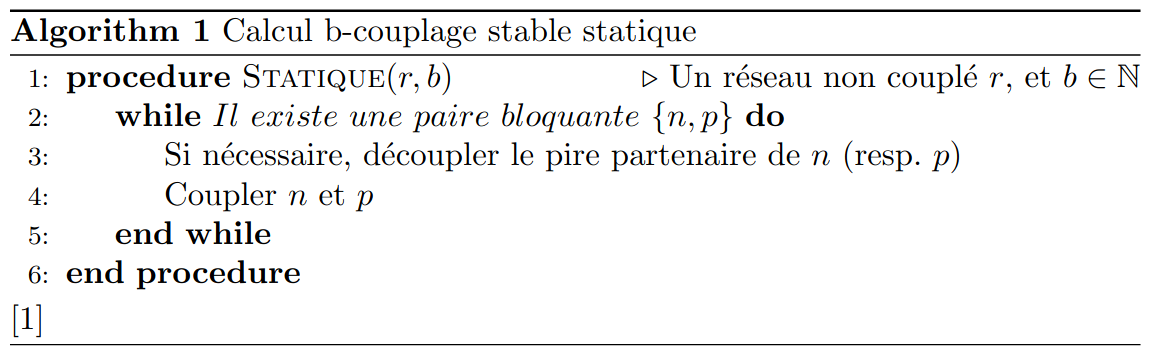
\includegraphics[width=0.8\linewidth]{algo1.png}
        \end{figure}
\end{frame}


\begin{frame}
    \frametitle{Couplage stable statique - Résultats}
        \begin{figure}
            \centering
            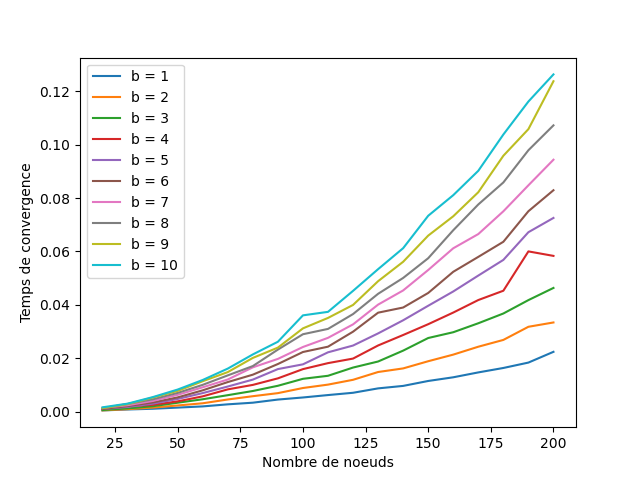
\includegraphics[width=0.7\linewidth]{chart_fab_p=1.png}
            \caption{Temps de convergence (s) de $STATIQUE$}
        \end{figure}
\end{frame}

\begin{frame}
    \frametitle{Couplage stable statique - Résultats}
        \begin{figure}
            \centering
            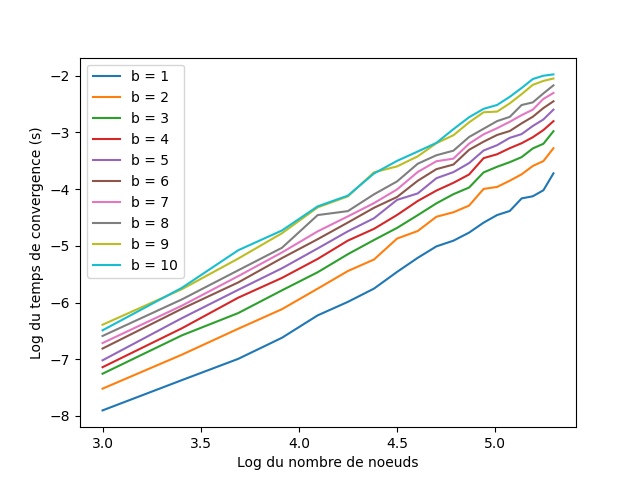
\includegraphics[width=0.7\linewidth]{chart_fab_log.png}
            \caption{Logarithme du temps de convergence de $STATIQUE$}
        \end{figure}
    \centering
    Complexité: $O(C_bn^a)$ où $a\simeq 2,5$
\end{frame}


% =================================================

\begin{frame}
    \frametitle{Couplage stable dynamique naïf}
    Description de l'algorithme:
    \begin{itemize}
        \item Construction d'un b-couplage stable
        \item A chaque modification, calcul d'un nouveau b-couplage stable via $STATIQUE$
    \end{itemize}
\end{frame}

\begin{frame}
    \frametitle{Couplage stable dynamique naïf - Résultats}
        \begin{figure}
            \centering
            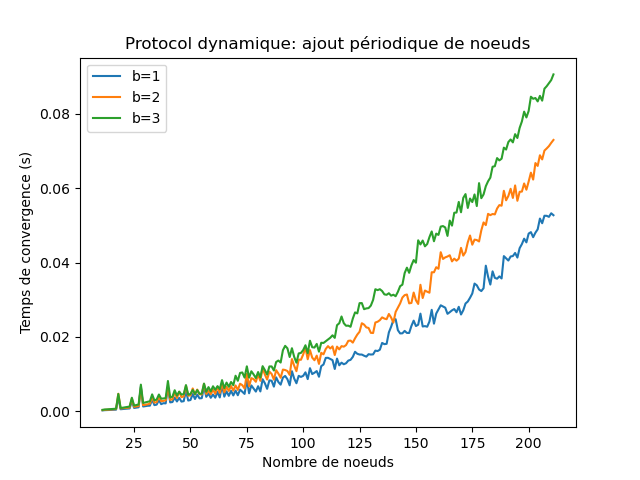
\includegraphics[width=0.7\linewidth]{chart_dyna_t.png}
            \caption{Ajout successifs de 200 noeuds à partir de $|R|=10$}
        \end{figure}
\end{frame}



% =================================================

\begin{frame}
    \frametitle{Calcul de couplage stable dynamique par modification locale}
    Description de l'algorithme:
    \begin{itemize}
        \item Construction d'un b-couplage stable
        \item A chaque modification, changement local du couplage autour de la modification
    \end{itemize}
    Mesure de satisfaction\footnote{\textit{Georgiadis \& Papatriantafilou, 2012}} pour un noeud $i$:
        \begin{equation}
            S_i = \frac{1}{b} . (c_i - \sum_{j}{\frac{R_j - C_j}{L_i}}) \in [0, 1]
        \end{equation}
    Elle quantifie la stabilité du couplage.
\end{frame}

\begin{frame}
    \frametitle{Méthode de modification locale - Mesure de satisfaction}   
    \begin{figure}
        \centering
        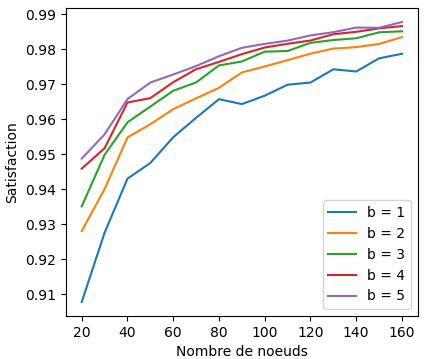
\includegraphics[width=0.7\linewidth]{chart_fab_sat.png}
        \caption{Satisfaction d'un couplage obtenu de $STATIQUE$}
    \end{figure}
\end{frame}

\begin{frame}
    \frametitle{Méthode de modification locale - Résultats}
    \begin{figure}
        \centering
        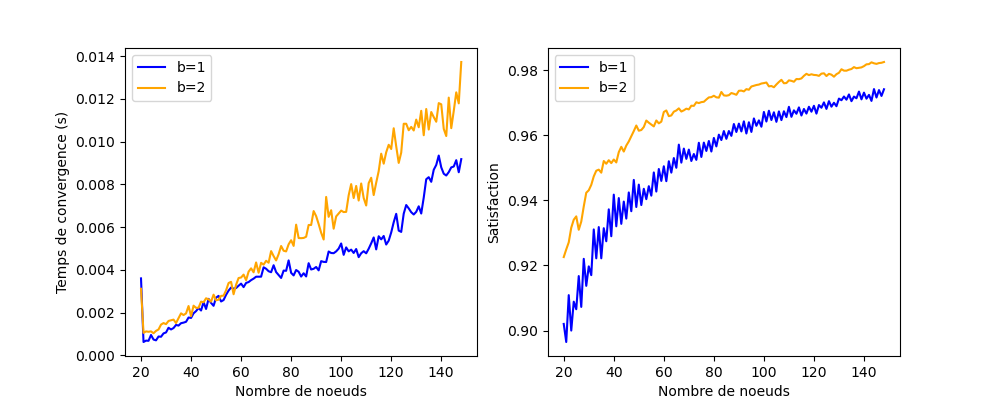
\includegraphics[width=0.9\linewidth]{chart_adap_add.png}
        \caption{Ajouts successifs de 130 noeuds à partir de $|R|=20$}
    \end{figure}
\end{frame}

\begin{frame}
    \frametitle{Méthode de modification locale - Résultats}
    \begin{figure}
        \centering
        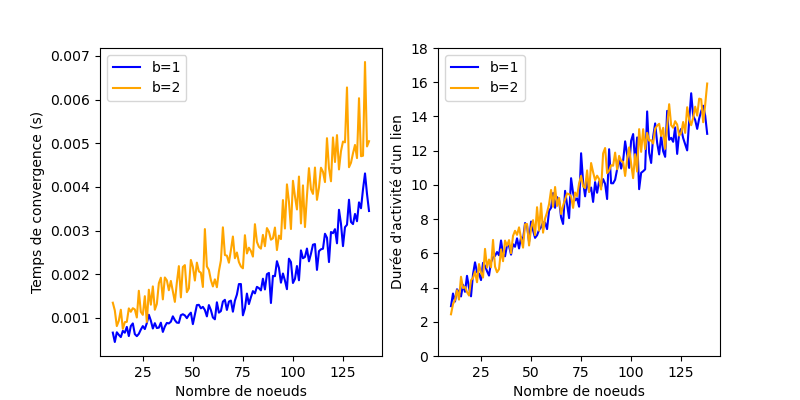
\includegraphics[width=0.8\linewidth]{chart_adap_t_span.png}
        \caption{Ajouts et retraits successifs à $|R|$ fixé}
    \end{figure}
\end{frame}


% =================================================



% =================================================

\begin{frame}
    \frametitle{Conclusions et perspectives}

    \begin{itemize}
        \item L'implémentation par couplages converge suffisamment rapidement
        \item La notion de satisfaction convient mieux que celle de couplage stable
        \item Perspectives: 
        \begin{itemize}
            \item Implémenter un algorithme réellement utilisé par les réseaux P2P $\rightarrow$ Comparaison
            \item Etude de cas limites
        \end{itemize}
    \end{itemize}

\end{frame}

% =================================================

\begin{frame}
    \frametitle{Bibliographie}

    \begin{thebibliography}{9}

        \bibitem{cohen} B. Cohen,
        \textit{The BitTorrent Protocol Specification},
        BitTorrent.org: BEP 3, 2008


        \bibitem{lebedev}
        D. Lebedev et al.,
        \textit{On Using Matching Theory to Understand P2P Network Design},
        International Network Optimization Conference, 2007


        \bibitem{mathieu}
        F. Mathieu,
        \textit{Self-stabilization in preference-based systems},
        Discrete Applied Mathematics, 2007

        \bibitem{papa}
        G. Georgiadis, M. Papatriantafilou
        \textit{Adaptive distributed b-matching in overlays with preferences},
        International Symposium on Experimental Algorithms, 2012

    \end{thebibliography}

\end{frame}

\begin{frame}
    \frametitle{Annexe 1 - Mesure de satisfaction}
    \begin{equation}
        S_i = \frac{1}{b} . (c_i - \sum_{j}{\frac{R_j - C_j}{L_i} \in [0, 1]}) \in [0, 1]
    \end{equation}
    $c_i$ : Nombre de noeuds couplés avec $i$

    $L_i$ : Longeur de la liste de préférence de $i$

    $R_j$ : Rang de $j$ dans la liste de préférence de $i$ 

    $C_j$ : Rang de $j$ parmi les noeuds couplés avec $i$
\end{frame}


\begin{frame}
    \frametitle{Annexe 2.1 - Condition d'acyclicité}
    Le graphe de préférence est désormais cyclique

    Description de l'algorithme:
    \begin{itemize}
        \item On retient les paires bloquantes parcourues
        \item Si on détecte un cycle, suppression d'un arête du cycle
        \item Si un noeud n'a plus d'arêtes, il est supprimé
    \end{itemize}
\end{frame}


\begin{frame}
\frametitle{Annexe 2.2 - Condition d'acyclicité}
\begin{figure}
    \centering
    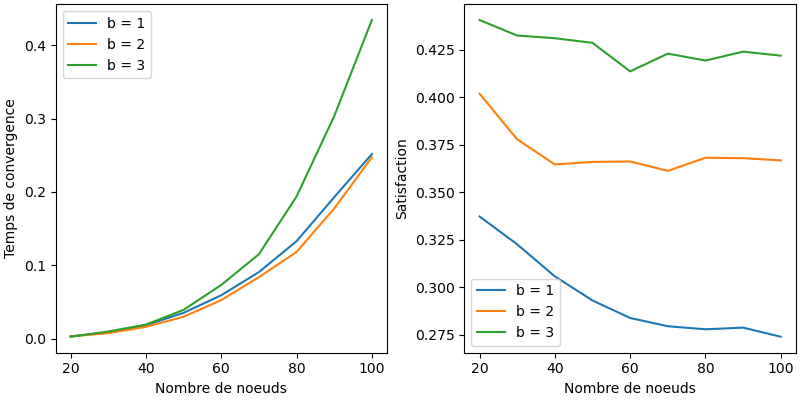
\includegraphics[width=0.9\linewidth]{chart_cyc_t_sat.png}
    \caption{Temps de convergence (s) et satisfaction de l'adaptation aux graphes de préférences cycliques}
    \end{figure}
\end{frame}

\begin{frame}[fragile]
    \frametitle{Annexe 3 - Code principal}
    \begin{verbatim}
    type trileen = Unmatched | Unloving | Loving
(*Différents états d’un noeud au sens d’une configuration*)

type node = {
    id: int;
    mutable ind_noeuds : int;
      (*indice du node dans le tableau reseau.noeuds *)
    mutable ind_unloving : int;
      (*indice du node dans reseau.unloving*)
    config : pfile;
      (* Tableau de noeuds rangé par marque décroissante des
      nodes avec lesquels le node peut échanger des données.
      C’est la liste d’adjacence de node dans le graphe
      d’acceptance. Les cases non utilisées sont à la fin du
      tableau et à None*)

    \end{verbatim}
\end{frame}

\begin{frame}[fragile]
    \begin{verbatim}
    couplage : pfile;
      (*Tableau de taille b ordonné par marque décroissante des
      nodes intervenant dans le couplage*)
    mutable num_loving : int;
      (*Nombre (majoré par b et par couplage.len) de peers au
      sein de couplage qui sont loving*)
}
and pfile = {
  (*Tableau trié selon la marque décroissante. Les cases non
  utilisées sont à None*)
    mutable tab : champ option array;
    mutable len : int;
}
and champ = { (*Modélise une arête depuis un noeud*)
    n : node;
    e : trileen;
      (*indique si node est dans le couplage ou pas*)
    marque : int;}
    \end{verbatim}
\end{frame}


\begin{frame}[fragile]
    \begin{verbatim}
type reseau = {
    mutable noeuds : node option array;
      (*tableau des nodes dans le réseau. Le node d’indice
      node.id est à l’indice node.id*)
    mutable len_noeuds : int;
      (*Taille de noeuds*)
    mutable len_unloving : int;
      (*Taille de unloving. Fin de l’algo quand ça atteint 0*)
    mutable unloving : node option array;
      (*tableau des noeuds dont le couplage n’est pas composé
      que de peers loving. La structure est la même que
      le tableau noeuds*)
}
    \end{verbatim}
\end{frame}


\begin{frame}[fragile]
    \begin{verbatim}
let couplement node peer reseau marque =
  (*On a trouvé une paire devant être couplée:
  On ajoute la paire au couplage et si la paire est
  loving on retire de chaque config le pair correspondant
  et on les enlève du unloving du réseau et on réduit le
  unloving du reseau si ils sont complètement couplés avec
  des loving*)
    pfile_insere node.couplage peer Unloving marque;
    pfile_insere peer.couplage node Unloving marque;
    set_flag_in_pfile node.config peer Unloving None;
    set_flag_in_pfile peer.config node Unloving None;
    match peer.config.tab.(peer.config.len -1) with
    | None -> (*Le peer choisi n’a pas de config\n"*)
        exit(1)
    | Some c when c.n.id = node.id -> (*La paire est loving*)
        traitement_loving node peer reseau
    | _ -> ()
    \end{verbatim}
\end{frame}

\begin{frame}[fragile]
    \begin{verbatim}
let traitement_loving node peer reseau =
  (*On effectue les démarches nécessaires pour coupler
  définitivement node et peer*)
    node.num_loving <- node.num_loving +1;
    peer.num_loving <- peer.num_loving +1;
    set_flag_in_pfile node.couplage peer Loving None;
    set_flag_in_pfile peer.couplage node Loving None;
    if node.num_loving = !b then (
      (*Le node est complètement couplé qu’avec des paires
      incassables: on le retire de unloving*)
        nullify_unloving reseau node;
        remove_from_couplages reseau node;)
    if peer.num_loving = !b then (
        nullify_unloving reseau peer;
        remove_from_couplages reseau peer;)
    rm_config node peer;
    rm_config peer node
    \end{verbatim}
\end{frame}

\begin{frame}[fragile]
    \begin{verbatim}
let protocol reseau =
    num.num <- 0;
    while reseau.len_unloving > 0 do
        initiative_best reseau;
    done

let connections_init p reseau =
  (*Génère une liste de préférence
  selon erdos-renyi*)
    let pf = pfile_vide () in
    for i = 0 to reseau.len_unloving -1 do
        match reseau.unloving.(i) with
        | None -> failwith "None au milieu du unloving"
        | Some node ->
            let m = rand_with_prob p in
            pfile_insere pf node Unmatched m;
    done;
    pf
    \end{verbatim}
\end{frame}


% -------------------------------------------------
\end{document}